\documentclass[9pt]{style/developercv}

% \edef \myLocation{\directlua{tex.sprint(os.getenv('LOCATION'))}}
% \edef \myCellPhone{\directlua{tex.sprint(os.getenv('CELL_NUMBER'))}}
% \edef \myEmailLink{\directlua{tex.sprint(os.getenv('EMAIL_LINK'))}}
% \edef \myEmail{\directlua{tex.sprint(os.getenv('EMAIL_DISPLAY'))}}
% \edef \myWebsiteLink{\directlua{tex.sprint(os.getenv('WEBSITE_LINK'))}}
% \edef \myWebsite{\directlua{tex.sprint(os.getenv('WEBSITE_DISPLAY'))}}
% \edef \myLinkedinLink{\directlua{tex.sprint(os.getenv('LINKEDIN_LINK'))}}
% \edef \myLinkedin{\directlua{tex.sprint(os.getenv('LINKEDIN_DISPLAY'))}}

\edef \myLocation{Koleczkowo}
\edef \myCellPhone{+48xxx}
\edef \myEmailLink{mailto:miotk.mikolaj@gmail.com}
\edef \myEmail{miotk.mikolaj@gmail.com}
% \edef \myWebsiteLink{\directlua{tex.sprint(os.getenv('WEBSITE_LINK'))}}
% \edef \myWebsite{\directlua{tex.sprint(os.getenv('WEBSITE_DISPLAY'))}}
\edef \myLinkedinLink{https://www.linkedin.com/in/miotkmikolaj/}
\edef \myLinkedin{miotkmikolaj}

\usepackage{graphicx}
\graphicspath{ {./imgs/} }
\begin{document}

%----------------------------------------------------------------------------------------
%	TITLE AND CONTACT INFORMATION
%----------------------------------------------------------------------------------------

\begin{minipage}[t]{0.45\textwidth}
  \vspace{-\baselineskip}
  \colorbox{black}{{\HUGE\textcolor{white}{\textbf{\MakeUppercase{Mikołaj}}}}}
  \colorbox{black}{{\HUGE\textcolor{white}{\textbf{\MakeUppercase{Miotk}}}}}
  \vspace{6pt}

	{\huge Technical Architect}
\end{minipage}
\begin{minipage}[t]{0.275\textwidth}
  \vspace{-\baselineskip}

	\icon{MapMarker}{12}{\myLocation}\\
	\icon{Phone}{12}{\myCellPhone} \\
  \icon{At}{12}{\href{\myEmailLink}{\myEmail}}\\
	\icon{Github}{12}{\href{https://github.com/mikeeq}{mikeeq}}\\
	\icon{Linkedin}{12}{\href{\myLinkedinLink}{\myLinkedin}}\\
\end{minipage}
\begin{minipage}[t]{0.275\textwidth}
  \vspace{-\baselineskip}

  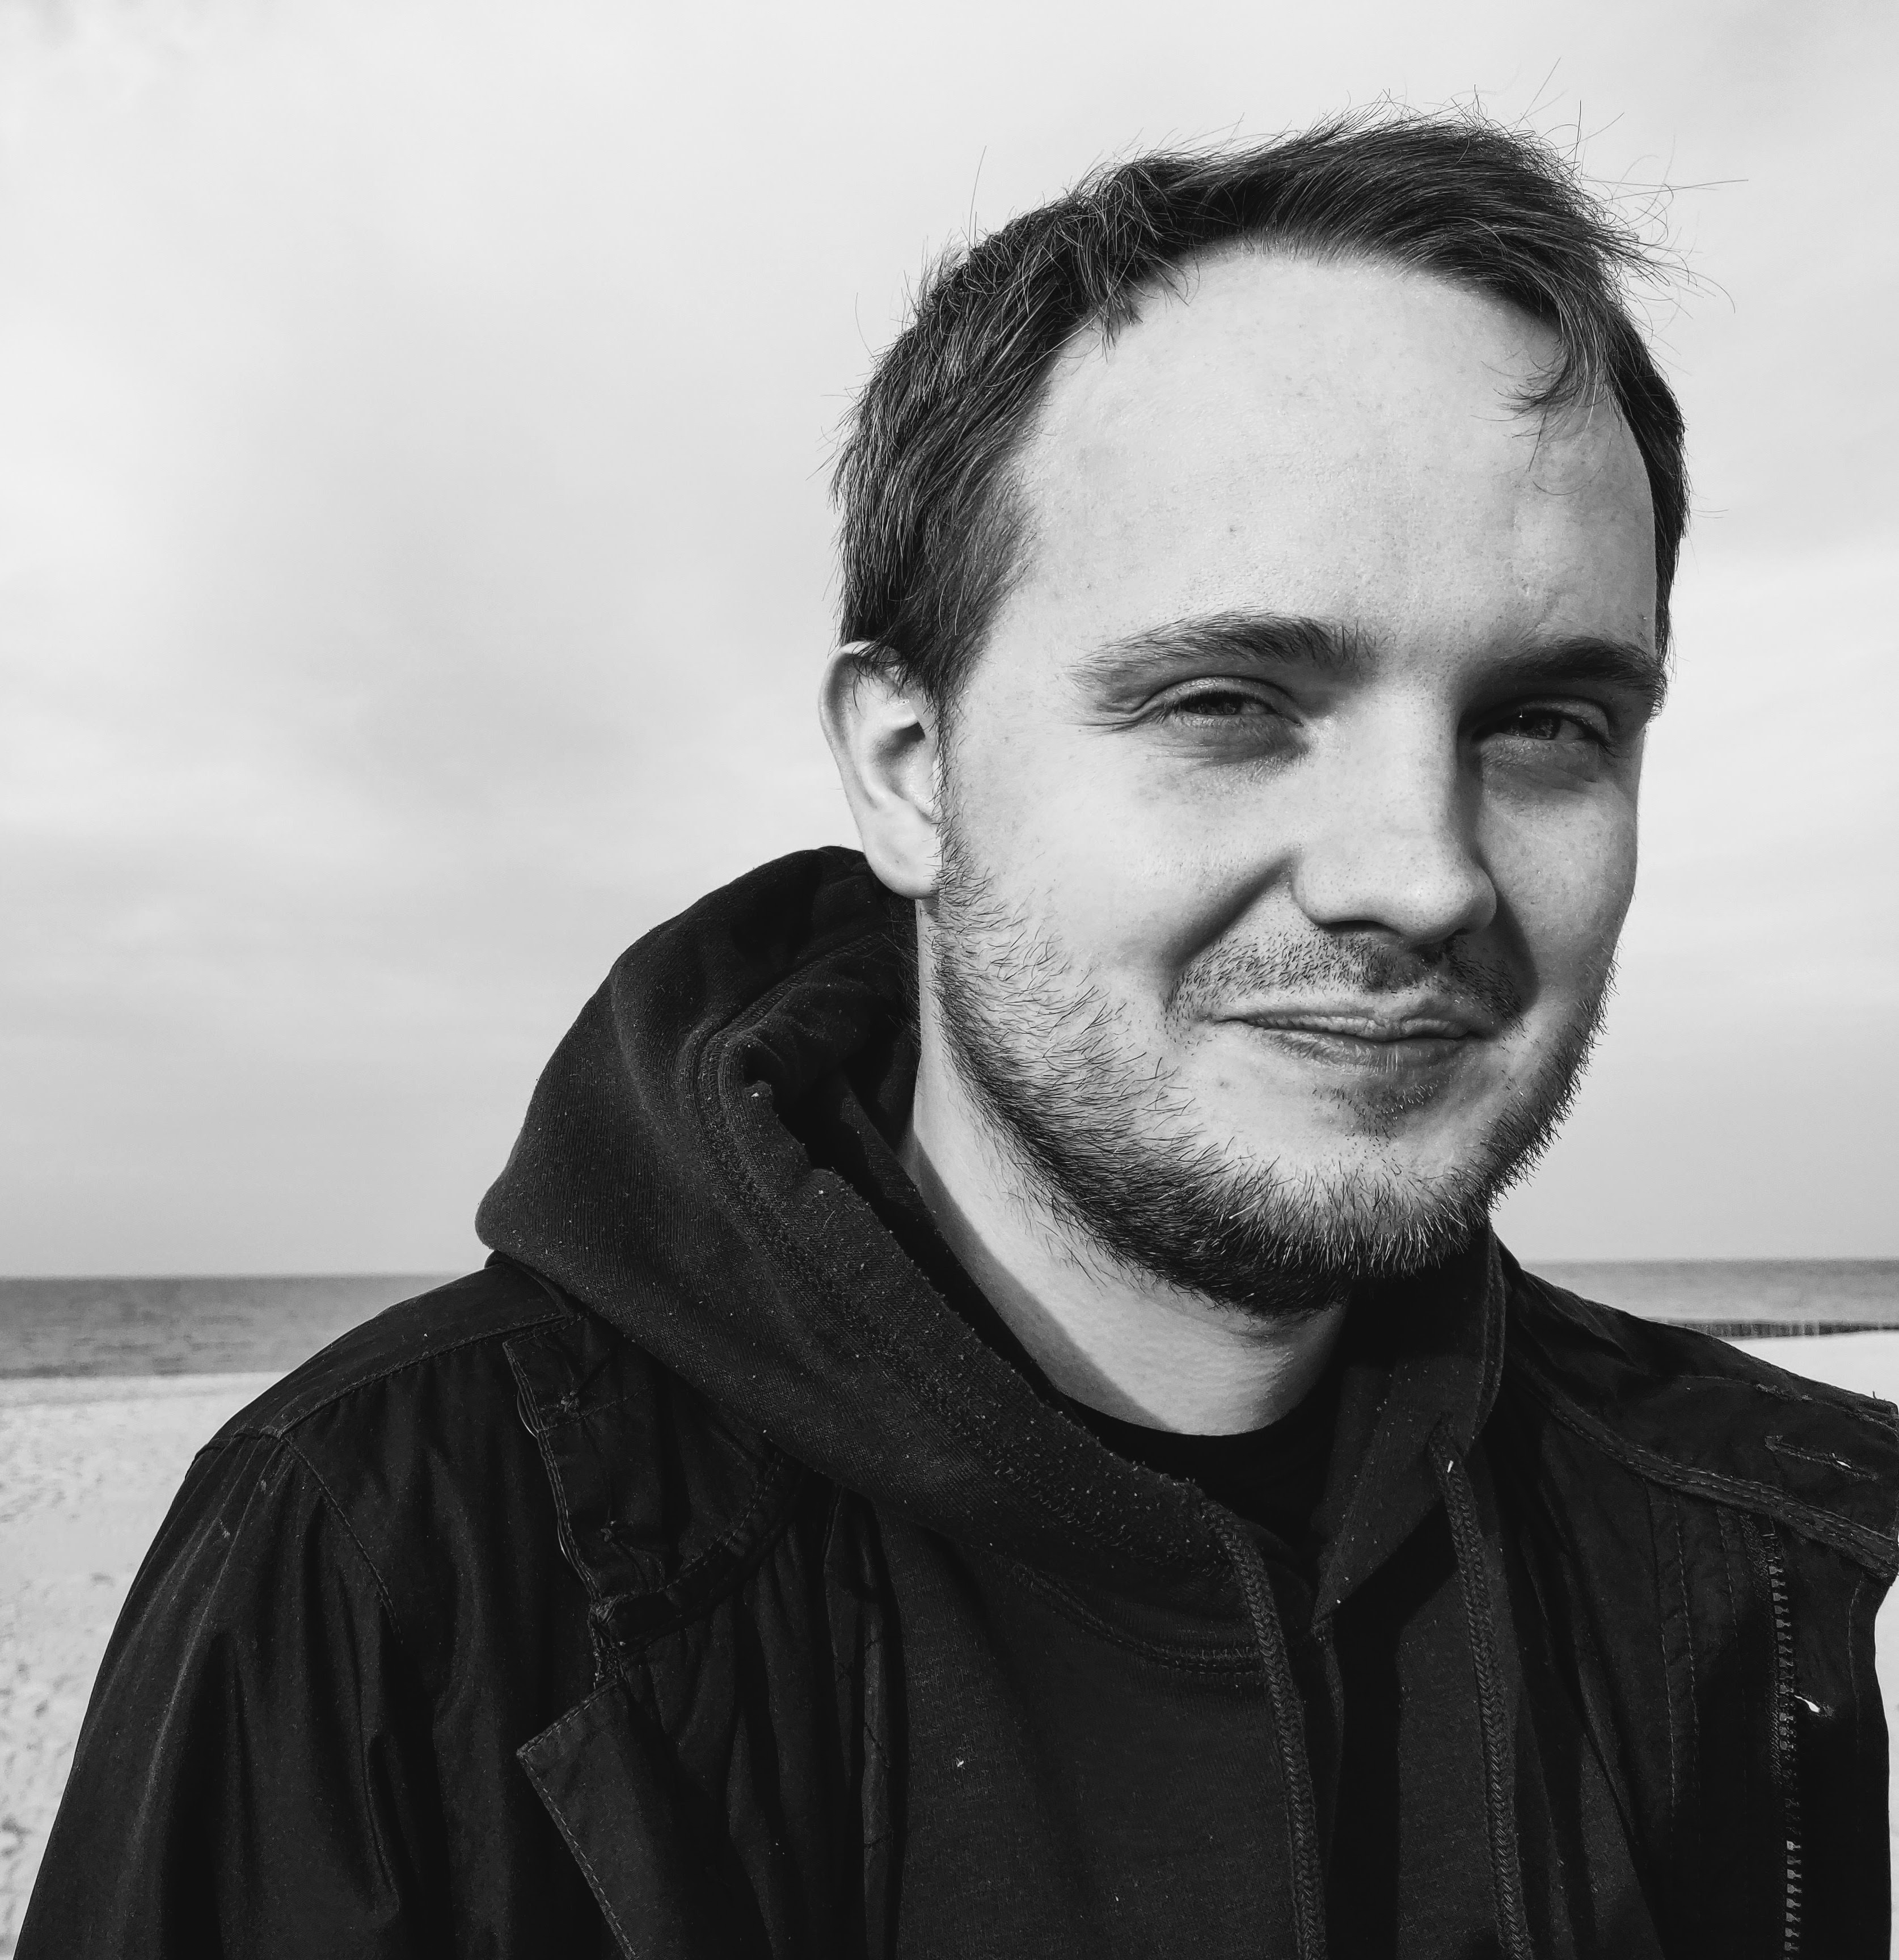
\includegraphics[scale=0.035]{photo_bw.jpg}
	% \icon{Globe}{12}{\href{\myWebsiteLink}{\myWebsite}}\\
	% \icon{Github}{12}{\href{https://github.com/mikeeq}{mikeeq}}\\
	% \icon{Linkedin}{12}{\href{\myLinkedinLink}{\myLinkedin}}\\
\end{minipage}

\vspace{0.5cm}

%----------------------------------------------------------------------------------------
%	INTRODUCTION, SKILLS AND TECHNOLOGIES
%----------------------------------------------------------------------------------------

\cvsect{Who Am I?}

\begin{minipage}[t]{0.4\textwidth} % 40% of the page width for the introduction text
	\vspace{-\baselineskip} % Required for vertically aligning minipages

  First and foremost, a computer enthusiast! I am a solution-oriented Technical Architect with over 9 years of professional IT experience.
  I specialise in designing scalable cloud platforms, DevOps automation, and enterprise architecture solutions.

\end{minipage}
\hfill % Whitespace between
\begin{minipage}[t]{0.5\textwidth} % 50% of the page for the skills bar chart
	\vspace{-\baselineskip} % Required for vertically aligning minipages
  \begin{barchart}{5.5}
    \baritem{Azure}{95}
    \baritem{CI/CD}{90}
		\baritem{Ansible}{90}
		\baritem{IaC}{85}
    \baritem{Docker}{85}
		\baritem{Kubernetes}{85}
	\end{barchart}
\end{minipage}

\vspace{1cm}

%----------------------------------------------------------------------------------------
%	TOP QUALITIES
%----------------------------------------------------------------------------------------

\begin{minipage}[t]{0.3\textwidth}
    \vspace{-\baselineskip}

    \cvsect{Collaborative}

  Knowledge sharing drives innovation - I regularly conduct technical workshops and mentoring sessions to elevate team capabilities and unblock complex architectural challenges.

\end{minipage}
\hfill
\begin{minipage}[t]{0.3\textwidth}
    \vspace{-\baselineskip}
    \cvsect{Strategic}

    Designing enterprise-grade solutions that align with business objectives whilst implementing industry best practices and ensuring optimal technology choices.

\end{minipage}
\hfill
\begin{minipage}[t]{0.3\textwidth}
    \vspace{-\baselineskip}
    \cvsect{Innovative}

  Continuously evaluating emerging technologies and architectural patterns to drive digital transformation and deliver measurable business value.

\end{minipage}
\vspace{0.75cm}

%----------------------------------------------------------------------------------------
%	EXPERIENCE
%----------------------------------------------------------------------------------------

\cvsect{Experience}
\begin{entrylist}
    \entry
    {Jun 2025 -- Present\\\footnotesize{Derby}
    \\Jun 2025  -- Present\\\footnotesize{Platform Technical Architect}}
        {Rolls-Royce - MMS migration}
        {Kainos}
        {
      \texttt{Azure DevOps}\slashsep
      \texttt{Azure CAF}\slashsep
      \texttt{Azure WAF}\slashsep
      \texttt{Azure Red Hat OpenShift ARO}\slashsep
      \texttt{IBM Maximo Application Suite}\slashsep
      \texttt{Oracle Database}\slashsep
      \texttt{Terraform}\\

      Architecting enterprise manufacturing system transformation through containerised IBM Maximo Application Suite deployment on Azure Red Hat OpenShift.\\
      \\
      Key Deliverables:\\
      - Designed OpenShift platform architecture for IBM MAS enterprise asset management\\
      - Architected Oracle Database integration strategy for manufacturing data\\
        }
    \entry
    {Nov 2024 -- Present\\\footnotesize{Derby}
    \\Nov 2024  -- Present\\\footnotesize{Platform Technical Architect}}
        {Rolls-Royce - FCC (Future Cloud Capabilities)}
        {Kainos}
        {
      \texttt{Azure DevOps}\slashsep
      \texttt{Azure CAF}\slashsep
      \texttt{Azure WAF}\slashsep
      \texttt{Azure Virtual Desktop AVD}\slashsep
      \texttt{Azure Migrate}\\

      Architected digital workplace transformation and cloud migration strategy for modern engineering infrastructure.\\
      \\
      Key Deliverables:\\
      - Designed Azure Virtual Desktop infrastructure for engineering workloads\\
      - Implemented Azure Migrate assessment and migration strategy for legacy systems\\
        }
    \entry
    {Oct 2023 -- Present\\\footnotesize{Remote}
    \\May 2023  -- Apr 2024\\\footnotesize{Platform Technical Architect}}
    {Royal London Group - Power Platform}
    {Kainos}
    {
      \texttt{Azure DevOps}\slashsep
      \texttt{Azure Well-Architected Framework}\slashsep
      \texttt{MS Power Platform}\slashsep
      \texttt{PowerBI}\slashsep
      \texttt{Power Platform CLI}\slashsep
      \texttt{Azure WAF}\slashsep
      \texttt{Data Gateway Architecture}\\

      Designed enterprise data platform architecture and CI/CD pipelines for Power Platform and PowerBI solutions following Azure Well-Architected Framework principles.\\
      \\
      Key Deliverables:\\
      - Architected CI/CD pipelines for Power Platform applications using Azure DevOps and Power Platform CLI\\
      - Designed automated PowerBI report deployment and governance workflows\\
      - Implemented solutions following Azure Well-Architected Framework's five pillars\\
      - Designed hybrid data gateway strategy for secure on-premises integration\\
    }
    \entry
    {Oct 2023 -- Present\\\footnotesize{Remote}
    \\Oct 2023  -- Apr 2024\\\footnotesize{Platform Technical Architect}}
        {Canada Life Group - Azure Landing Zone deployment}
        {Kainos}
        {
            \texttt{Azure CAF}\slashsep
      \texttt{Azure Landing Zone}\slashsep
            \texttt{Azure Firewall}\\

      Architected cloud foundation and security framework for financial services transformation.\\
      \\
      Key Deliverables:\\
      - Designed Azure Landing Zone architecture following CAF principles\\
      - Implemented enterprise-grade network security architecture\\
      - Established cloud governance and compliance frameworks\\
        }
    \entry
    {Jun 2021 -- Sep 2023\\\footnotesize{Gdynia}
    \\Jun 2021 -- Sep 2023\\\footnotesize{DevOps Consultant}}
        {DNV - GSS IT Kubernetes Platform}
        {JIT Team}
        {
            \texttt{Azure}\slashsep
      \texttt{AKS}\slashsep
            \texttt{Kubernetes}\slashsep
            \texttt{Istio}\slashsep
            \texttt{Velero}\slashsep
      \texttt{Prometheus}\slashsep
      \texttt{Loki}\slashsep
      \texttt{Kubecost}\slashsep
      \texttt{ArgoCD}\slashsep
      \texttt{F5 WAF}\slashsep
      \texttt{Victoria Metrics}\\

      Architected and delivered enterprise multi-tenant Kubernetes platform serving development teams across DNV's global organisation.\\
      \\
      Key Deliverables:\\
      - Designed cloud-native platform architecture with service mesh capabilities\\
      - Implemented GitOps-based deployment strategy using ArgoCD\\
      - Architected observability stack with cost optimisation features\\
        }
    \entry
    {Oct 2020 -- May 2021\\\footnotesize{Gdynia}
    \\Oct 2020 -- May 2021\\\footnotesize{DevOps Consultant}}
        {DNV GL - GSS IT Monitoring}
        {JIT Team}
        {
            \texttt{Azure}\slashsep
      \texttt{AKS}\slashsep
            \texttt{Azure Monitor}\slashsep
            \texttt{Azure Log Analytics}\slashsep
            \texttt{Azure DevOps}\slashsep
      \texttt{Ansible}\slashsep
      \texttt{Terraform}\\

      Designed automated monitoring platform architecture enabling centralised observability across DNV's global infrastructure.\\
      \\
      Key Deliverables:\\
      - Architected tag-based Azure Monitor deployment automation\\
      - Designed scalable alerting and dashboard provisioning strategy\\
      - Implemented Infrastructure as Code practices for monitoring stack\\
        }
    \entry
    {Mar 2018 -- Sep 2020\\\footnotesize{Leeds}
    \\Sep 2018 -- Sep 2020\\\footnotesize{Senior Ops Engineer}
    \\Mar 2018 -- Sep 2018\\\footnotesize{Associate WebOps Engineer}}
        {NHS Digital - NHS App}
        {Kainos}
        {
            \texttt{Azure}\slashsep
      \texttt{Kubernetes}\slashsep
      \texttt{AKS}\slashsep
            \texttt{Helm}\slashsep
            \texttt{Splunk}\slashsep
            \texttt{TeamCity}\slashsep
            \texttt{Azure DevOps}\slashsep
      \texttt{Terraform}\\
      \texttt{URL: \underline{https://www.nhs.uk/using-the-nhs/nhs-services/the-nhs-app/}}\\

      Designed and implemented cloud platform architecture for public healthcare application serving millions of UK citizens.\\
      \\
      Key Deliverables:\\
      - Architected secure, compliant Kubernetes platform for healthcare data\\
      - Designed CI/CD pipeline architecture with automated security scanning\\
      - Implemented centralised logging platform using Splunk Enterprise\\
        }
	\entry
    {Jul 2017 -- Feb 2018\\\footnotesize{London}
    \\Sep 2017 -- Feb 2018\\\footnotesize{Associate WebOps Engineer}
    \\Jul 2017 -- Sep 2017\\\footnotesize{Trainee WebOps Engineer}}
		{Ministry of Justice HMPPS - Digital Prisons}
		{Kainos}
		{
			\texttt{Azure}\slashsep
			\texttt{Windows Server}\slashsep
			\texttt{RDS}\slashsep
			\texttt{Ansible}\slashsep
			\texttt{Powershell DSC}\slashsep
      \texttt{Jenkins}\\
      \texttt{Terraform}\\

      Cloud-based kiosk self-service for prisoners and prison staff. \\
      \\
      Responsibilities:\\
      - Creating automated packaging/deployment solutions based on Chocolatey and Ansible\\
      - Building automation for creating/managing Windows Server Remote Desktop Services HA IaaS clusters.

		}
	\entry
    {May 2017 -- Jun 2017\\\footnotesize{Gdańsk}\\
    \footnotesize{Trainee WebOps Engineer}}
		{WebOps Academy}
		{Kainos}
		{
			\texttt{Azure}\slashsep
			\texttt{AWS}\slashsep
			\texttt{Puppet}\slashsep
			\texttt{Vagrant}\slashsep
			\texttt{Packer}\slashsep
			\texttt{Jenkins}\slashsep
			\texttt{Grafana}\\

      Corporate/internal series of workshops and training sessions.
		}
	\entry
		{Feb 2017 -- Apr 2017\\\footnotesize{Gdańsk}}
		{Software Engineer Intern in Cloud Computing (Reference Architectures team)}
		{Intel Corporation Poland}
		{
      \texttt{Azure Stack}\slashsep
      \texttt{Azure Service Fabric}\slashsep
      \texttt{Hyper-V}\slashsep
      \texttt{Docker}\slashsep
			\texttt{Windows Server Native Containers}\slashsep
			\texttt{CoreOS}\\

      Research and development of hybrid cloud architecture solutions for enterprise customers.\\
      \\
      Key Deliverables:\\
      - Designed proof-of-concept for containerised SQL Server on Azure Stack\\
      - Implemented monitoring architecture using InfluxDB and Grafana\\

		}
	\entry
    {Jul 2016 -- Jan 2017\\\footnotesize{Gdańsk}}
		{Operator IT}
		{Grupa Wirtualna Polska}
		{
			\texttt{Zabbix}\slashsep
			\texttt{RedHat Linux}\slashsep
			\texttt{Hardware Maintenance}\\

      Maintained production infrastructure and monitoring systems for high-traffic web services.\\
      \\
      Key Responsibilities:\\
      - Provided 2nd/3rd line support for critical production systems\\
      - Enhanced monitoring capabilities and incident response procedures\\
		}
	\entry
    {Apr 2016 -- Jul 2023\\\footnotesize{Gdańsk}}
    {Local Network Administrator}
    {Gdańsk University of Technology}
		{
			\texttt{CentOS}\slashsep
			\texttt{HP ProCurve}\slashsep
			\texttt{Puppet}\slashsep
			\texttt{Zabbix}\\
      \texttt{URL: https://pg.edu.pl/en/sccn}\\

      Maintained network infrastructure serving university campus community.\\
      \\
      Key Responsibilities:\\
      - Architected high-availability network infrastructure for student accommodation\\
      - Implemented automated configuration management and monitoring systems\\
      - Led knowledge transfer initiatives across technical teams\\
		}
\end{entrylist}

%----------------------------------------------------------------------------------------
%	EDUCATION
%----------------------------------------------------------------------------------------

\cvsect{Education}

\begin{entrylist}
	\entry
		{2013 -- 2020}
    {Bachelor of Engineering}
    {Gdańsk University of Technology}
    {
      \texttt{OpenStack}\slashsep
      \texttt{Terraform}\slashsep
      \texttt{GitLab CI}\slashsep
			\texttt{Kubernetes}\slashsep
			\texttt{Kubespray}\slashsep
			\texttt{Helm}\\

      \textbf{Field of Study}: Electronics and Telecommunications, \\
      \textbf{Stream}: Telecommunications,\\
      \textbf{Specialization}: Radio Communication systems and networks,\\
      \textbf{Thesis}: Creation of the platform for orchestration NLP services used by plagiarism detection system\\
    }
		{}
\end{entrylist}

%----------------------------------------------------------------------------------------
%	ADDITIONAL INFORMATION
%----------------------------------------------------------------------------------------

\begin{minipage}[t]{0.3\textwidth}
	\vspace{-\baselineskip}

	\cvsect{Languages}

	\textbf{English} - proficient\\
	\textbf{Polish} - native
\end{minipage}
\hfill
\begin{minipage}[t]{0.3\textwidth}
	\vspace{-\baselineskip}

	\cvsect{Hobbies}

  Automobiles\\
  Retro Video Games/Consoles\\
  Sports\\
  Technology
\end{minipage}
\hfill
\begin{minipage}[t]{0.3\textwidth}
	\vspace{-\baselineskip}

	\cvsect{Personal Side Projects}

  \textbf{mbp-fedora} - first Linux distribution build with full Apple T2 compatibility (newer Intel-based Macs)\\
  \textbf{xiaomi-ax3200-openwrt} - tutorial and first builds of OpenWRT images for Xiaomi Wi-Fi 6 router\\
  \textbf{ansible-ops-workstation} - automation for configuring Fedora and Ubuntu workstations

\end{minipage}
% \hfill
% \begin{minipage}[t]{0.3\textwidth}
% 	\vspace{-\baselineskip}

% 	\cvsect{Certificates}

  % CKA
% \end{minipage}

%----------------------------------------------------------------------------------------

\vspace{1.00cm}

\begin{minipage}[t]{1\textwidth}
	I hereby agree to the processing of personal data provided in this document for
	realising the recruitment process pursuant to the Personal Data Protection Act
	of 10 May 2018 (Journal of Laws 2018, item 1000) and in agreement with Regulation (EU)
	2016/679 of the European Parliament and of the Council of 27 April 2016 on the
	protection of natural persons with regard to the processing of personal data and on
	the free movement of such data, and repealing Directive 95/46/EC (General Data
	Protection Regulation).
\end{minipage}

\end{document}
